% 中点四边形 例3：原四边形对角线相等且垂直 -> 中点四边形是正方形
\documentclass[tikz,border=4pt]{standalone}
\usepackage{ctex}
\usepackage{amsmath}
\usetikzlibrary{calc}
\begin{document}
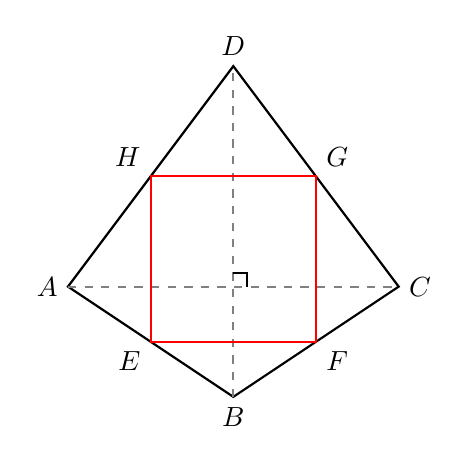
\begin{tikzpicture}[scale=0.7, thick]
  % 选: AC 水平, BD 垂直, 长度都为 6, 不对称分割
  % AC: A=(-2,0), C=(4,0), len=6
  % BD: 过中点不规则 - 让它们在某点垂直相交即可。设交点 P=(1,0).
  % B=(1,-2), D=(1,4). BD=6, AC=6, 垂直相交于 P=(1,0).
  \coordinate (A) at (-2,0);
  \coordinate (B) at (1,-2);
  \coordinate (C) at (4,0);
  \coordinate (D) at (1,4);
  \coordinate (E) at ($(A)!0.5!(B)$);
  \coordinate (F) at ($(B)!0.5!(C)$);
  \coordinate (G) at ($(C)!0.5!(D)$);
  \coordinate (H) at ($(D)!0.5!(A)$);
  \draw (A)--(B)--(C)--(D)--cycle;
  \draw[gray, dashed] (A)--(C);
  \draw[gray, dashed] (B)--(D);
  \draw[red] (E)--(F)--(G)--(H)--cycle;
  % 直角 AC ⊥ BD
  \draw ($(1,0)+(0.25,0)$)--($(1,0)+(0.25,0.25)$)--($(1,0)+(0,0.25)$);
  \node[left] at (A) {$A$};
  \node[below] at (B) {$B$};
  \node[right] at (C) {$C$};
  \node[above] at (D) {$D$};
  \node[below left] at (E) {$E$};
  \node[below right] at (F) {$F$};
  \node[above right] at (G) {$G$};
  \node[above left] at (H) {$H$};
\end{tikzpicture}
\end{document}
